\documentclass[thesis]{subfiles}

\begin{document}

\def\cxx{{C\nolinebreak[4]\hspace{-.05em}\raisebox{.3ex}{\footnotesize ++}}\xspace}

\OnlyInSubfile{\setcounter{chapter}{5}}

\chapter{Implementation of molecular simulation software}

\vskip\baselineskip

During my PhD, I also worked to implement molecular simulation software as part
of the domino project. In this chapter I will this project and my contributions
to it, as well as some advanced simulation techniques I worked to incorporate in
domino.

The first of these advanced methods is the Hybrid Monte Carlo simulation
technique, which join molecular dynamics and Monte Carlo in an attempt to get
the advantages of both. I will present the original method and some of the most
recent developments and improvements to it.

The second of these methods concern the treatment of electrostatic interactions
in the context of periodic boundary conditions. I will first describe the Ewald
summation technique, and some tricks for optimizing its implementation. Then I
will discuss the Wolf summation method as one alternative to Ewald summation
that only relies on a sum of pair terms.

\newpage
\section{Domino: extensible molecular simulations library}

\cxx, scientific software.

\cxx11 => common, can make it fast, simple subset

Assume basic \cxx and object-oriented knowledge from reader

\subsection{Goals and architecture}

=> extensible, mixed MC/MD

=> classical only

=> library

Pure virtual classes, no deep hierarchy

Inherit and implement as an extension strategy

Library vs framework

Example for MD NPT and MC uVT

\subsubsection{Contributions to Domino}

Code quality:

cleanup + modernizing code

Add tests with reference NIST data

Potential interface

YAML for input

System representation and normalization



Algorithms:

GCMC

Hybrid Monte Carlo

Anisotropic Stress tensor

Berendsen anisotropic barostat

Monte-Carlo barostat

CSVR thermostat

Ewald

Wolf

\subsection{Challenges of mixed simulation software}

=> MD + MC

=> on demand computation of forces + energy

\subsubsection{Computing pressure and stress}

\subsection{Monte Carlo energy caching}

Pairs + Ewald

All moves


\newpage
\section{Hybrid Monte Carlo}
\label{sec:hmc}

\emph{Hybrid Monte Carlo}, also called \emph{Hamiltonian Monte Carlo} (HMC) is
an improvement on standard Metropolis Monte Carlo that allow to simulate complex
systems more efficiently. Considering a Monte Carlo in the $NVT$ ensemble, the
usual way to generate new conformation for the Markov chain is to randomly pick
and translate (and additionally rotate for rigid molecules) a particle in the
system. The amplitude of the translation is limited by the move acceptance rate:
while higher amplitudes allow to sample the phase space more efficiently, they
are correlated with a much lower acceptance rate; and thus increase the amount
of work done by the simulation to generate a new conformation.

This is even more relevant when the system contains large flexible molecules,
spanning long distances, such as proteins, polymers or here, metal--organic
frameworks. The typical movements and conformation changes of the molecule are
by nature collective, multiple atoms moving together in the same direction. The
standard Monte Carlo moves have difficulties to sample these kind of collective
behaviors, as they would require multiple single atom moves in the same
direction. Multiple improved Monte Carlo moves have been proposed to overcome
these limitations. For small molecules displaying intra-molecular flexibility,
it is possible to directly sample rotations around all the bonds using
configuration bias Monte Carlo base on Rosenbluth sampling (see
reference~\cite{Frenkel1997} for more details on the algorithm), where the
molecule is fully regrown from a starting atom, randomly choosing the
orientation of the next backbone bond at each step.  This procedure is
illustrated in figure~\ref{fig:cbmc}.

\begin{figure}[ht]
    \centering
    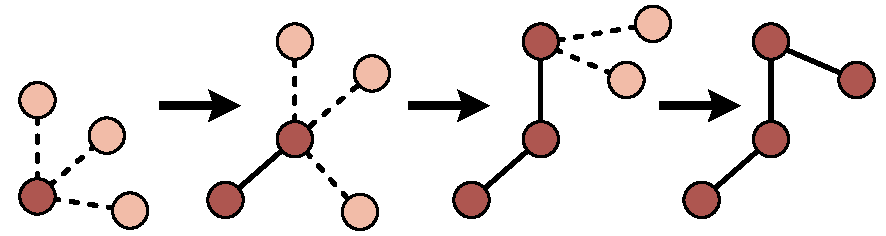
\includegraphics[width=0.8\textwidth]{figures/images/cbmc}
    \caption{Illustration of a single configurational bias Monte Carlo move. A
    linear molecule is regrown step by step. At each step, the position for the
    next atom is picked at random, depending on the position of all the
    previous atoms.}
    \label{fig:cbmc}
\end{figure}

The main issues with configuration bias Monte Carlo is that it requires
knowledge of all the separated intra-molecular interaction terms to be able to
generate the position of the next atom while maintaining detailed balance; and
not only the global energy change as for simpler moves. It is also harder to use
it for even the simplest branched molecules.

Flexible nanoporous materials add another level of difficulty for efficient
Monte Carlo simulations. Some of them display collective behavior linked to
global deformations of the simulation cell, such as breathing in MIL-53 or some
cases of gate-opening. Here, the volume of the simulation cell changes as the
linkers rotate and move, thus needing Monte Carlo moves able to sample both the
collective rotation of linkers and the changes in the unit cell shape and
volume. It is possible to use molecular dynamics instead of Monte Carlo to
explore the response of the material to an external stress, as molecular
dynamics simulations are very efficient when sampling collective behaviors. But
when the stress is created by adsorbed molecules, we need to use grand canonical
Monte Carlo (see section~\ref{sec:gcmd}). Hybrid Monte Carlo is a technique that
can bridge the gap between traditional Monte Carlo and molecular dynamics,
bringing the ability to sample such collective motions to a Monte Carlo
simulation\cite{Rogge2019}.

In addition to being able to improve the sampling efficiency of Monte Carlo
simulations, Hybrid Monte Carlo can bring the power of non-physical moves in
simulations usually relying on molecular dynamics. For example, the study of
large bio-molecules --- the typical example is the simulation of protein folding
--- is often limited by the time scale at which the simulation can produce a new
conformation, decorrelated from the previous one\cite{Izaguirre2004}. Monte
Carlo can help to reduce this time by allowing jump from one conformation to
another, and incorporate domain specific knowledge (which part of the protein
can rotate, which parts will move together) to improve simulation efficiency.

Another area that can see improvements by incorporating non-physical moves is
the simulation of diluted aqueous environment, such as the salt and pH
environment around proteins. The pH of human blood is constant around 7.4,
meaning that both \ce{HO-} and \ce{H+} ions are only present at concentration
around \SI{e-7}{mol/L}. If we want to simulate a realistic pH environment, we
need to simulate more than 500 million water molecule for each \ce{HO-} or
\ce{H+} ion. In addition to that, because the surface of proteins can carry
non-neutral charges, the local ion concentration can depart from the measured,
global concentration in blood plasma or cell's cytoplasm. Grand Canonical and
semi-Grand Canonical Monte Carlo moves used together with Hybrid Monte Carlo can
bring realistic salt and pH condition to these simulations\cite{Ross2018}.

\subsection{Mixing molecular dynamics and Monte Carlo}

Hybrid Monte Carlo was first devised in 1987 by \citeauthor{Duane1987} for
calculations in lattice quantum chromodynamics \cite{Duane1987}. It was then
adapted to condensed matter molecular simulation by \citeauthor{Mehlig1992} in
1992\cite{Mehlig1992}. The central idea is to use a short molecular dynamics
simulation (around 10 steps) to generate a new conformation for the Markov
chain. Once the molecular dynamics simulation finished, the final step is
considered as a trial conformation, and accepted or rejected with the adapted
Metropolis criterion.

One global move in \emph{configuration space} consists in propagating the system
through \emph{phase space} for a fixed number of steps using some integration
scheme $\psi_{\delta t}$ of Hamilton's equations. $\psi_{\delta t}$ depends on
the integration time step $\delta t$ and the Hamiltonian of the system
$\mathcal{H}$; and maps the initial configuration $(\r, \v)$ in phase space to
the final one $(\r', \v')$:
\[\begin{array}{llcl}
    \psi_{\delta t} : & \mathbb{R}^{6N} & \longrightarrow & \mathbb{R}^{6N} \\
                      & (\r, \v)        & \longmapsto     & \psi_{\delta t}(\r, \v) \equiv (\r', \v')
\end{array}\]

Since the usual Monte Carlo scheme does not uses the atomic velocities, we need
to generate new velocities before starting the molecular dynamics simulation. We
choose to generate them according the the canonical ensemble distribution at
temperature $T$:
\[ \mathcal{P}_T(\v) \propto \exp\left(- \beta \sum_i \frac 12 m_i \v_i^2 \right)\]

Following the same notations as in chapter~\ref{sec:molsim}, because the time
integration is deterministic, the probability $\alpha(\r \to \r')$ to generate a
given conformation $\r'$ starting from $\r$ is the same as the probability to
generate a specific set of initial velocities $\mathcal{P}_T(\v)$:
\[ \alpha(\r \to \r')\ \d\r' = \mathcal{P}_T(\v) \ \d\v \]

If we use an acceptation probability that depends on the discretization error
$\delta \mathcal{H}$:
\begin{gather}
    \text{acc}((\r, \v) \to (\r', \v')) = \min\left(1, e^{-\beta \delta \mathcal{H}}\right), \\
    \delta \mathcal{H} = \mathcal{H}(\r', \v') - \mathcal{H}(\r, \v);
\end{gather}
we can show that the resulting Monte Carlo move respect the detailed balance
provided that the integration scheme $\psi_{\delta t}$ is \emph{time reversible}
and \emph{symplectic}.
\[\begin{array}{lcl}
    \mathcal{P}(\r)\ \pi(\r \to \r') \ \d\r\d\v   &=& \mathcal{P}(\r)\ \mathcal{P}_T(\v)\ \text{acc}\kern-0.5ex\left((\r, \v) \to \psi_{\delta t}(\r, \v)\right) \d\r\d\v \\
    \text{\footnotesize \itshape see below}       &=& \mathcal{P}(\r')\ \mathcal{P}_T(\v')\ \text{acc}\kern-0.5ex\left(\psi_{\delta t}(\r, \v) \to (\r, \v)\right) \d\r\d\v \\
    \text{\footnotesize \itshape time reversible} &=& \mathcal{P}(\r')\ \mathcal{P}_T(\v')\ \text{acc}\kern-0.5ex\left((\r', \v') \to \psi_{-\delta t}(\r', \v')\right) \d\r\d\v \\
    \text{\footnotesize \itshape symplectic}      &=& \mathcal{P}(\r')\ \mathcal{P}_T(\v')\ \text{acc}\kern-0.5ex\left((\r', \v') \to \psi_{-\delta t}(\r', \v')\right) \d\r'\d\v' \\
    \mathcal{P}(\r)\ \pi(\r \to \r') \ \d\r\d\v &=& \mathcal{P}(\r')\ \pi(\r' \to \r) \ \d\r'\d\v'
\end{array}\]
The first step in the above demonstration comes from the mathematical identity
\[e^{-\beta\mathcal{H}(\r, \v)} \min\kern-0.5ex\left(1, e^{-\beta \delta \mathcal{H}}\right) = e^{-\beta\mathcal{H}(\r', \v')} \min\kern-0.5ex\left(e^{\, \beta \delta \mathcal{H}}, 1\right). \]

It is worth noting that even though the molecular dynamics simulation evolves in
the micro-canonical $NVE$ ensemble, the overall HMC simulation is sampling the
canonical $NVT$ ensemble. This allow to use HMC simulations as a rigorous way to
sample the $NVT$ ensemble using molecular dynamics.

The acceptance rate of the hybrid moves is dictated by the value of
$\delta\mathcal{H}$. This value is the discretization error associated with the
timestep used by the molecular simulation, and depends only on $\delta t$ and
the number of steps used to propagate the system with molecular dynamics. These
are the parameters we can adjust to change the global acceptance rate.

\subsection{Related algorithms and methods}

In the last decade, improvements

Since the original hybrid Monte Carlo method

\subsubsection{Shadow Hybrid Monte Carlo}

\subsubsection{Compressible Hybrid Monte Carlo}

\subsubsection{Constant pressure Hybrid Monte Carlo}


\TODO\cite{Akhmatskaya2009}

\TODO\cite{Izaguirre2004}

\TODO\cite{Akhmatskaya2011}

\TODO\cite{Fang2014}

\subsection{Sampling other ensembles}

\TODO constant pressure simulation

\TODO osmotic simulations\cite{Rogge2019}

\subsection{Hybrid simulations of adsorption}

I used my implementation of hybrid Monte Carlo in domino to study adsorption of
methane \ce{CH4} in MOF-5 at \SI{300}{K}. I used a simplified model of both
MOF-5 and \ce{CH4} as domino did not support computing electrostatic
interactions at the time. \ce{CH4} molecules where approximated by a single
spherical Lennard-Jones sphere, using $\sigma = \SI{3.737}{\AA}$ and $\epsilon =
\SI{1.247}{kJ/mol}$. I used the Lennard-Jones and intra-molecular terms from
QuickFF\cite{Vanduyfhuys2015}, ignoring the atomic charges. While the resulting
model is not an accurate representation of MOF-5, it is still an interesting
test case for the use of hybrid Monte Carlo simulations in adsorption.

To obtain a full isotherm , I ran 8 simulations at different \ce{CH4} pressures.
Each simulation used two Monte Carlo moves: insertion/deletion of \ce{CH4}
taking the current pressure as the gas fugacity; and hybrid moves. The hybrid
moves used a Velocity-Verlet integrator with a timestep of \SI{1}{fs}, and a
Berendsen barostat setting the external pressure at the same value as the
\ce{CH4} fugacity and a time step of \SI{5}{ps}. I should point out that I used
the Berendsen barostat even if it is not symplectic nor time reversible, as it
was the only barostat implemented in domino. Again, while the resulting
simulation might not sample the adequate ensemble, it is still and interesting
check. Each simulation was propagated for a million of Monte Carlo moves, using
the first 250 000 moves as the equilibration period. The resulting isotherms is
shown in figure~\ref{fig:hmc-mof5} together with the changes in volume as the
pressure increases.

\begin{figure}[ht]
    \centering
    % GNUPLOT: LaTeX picture with Postscript
\begingroup
  \makeatletter
  \providecommand\color[2][]{%
    \GenericError{(gnuplot) \space\space\space\@spaces}{%
      Package color not loaded in conjunction with
      terminal option `colourtext'%
    }{See the gnuplot documentation for explanation.%
    }{Either use 'blacktext' in gnuplot or load the package
      color.sty in LaTeX.}%
    \renewcommand\color[2][]{}%
  }%
  \providecommand\includegraphics[2][]{%
    \GenericError{(gnuplot) \space\space\space\@spaces}{%
      Package graphicx or graphics not loaded%
    }{See the gnuplot documentation for explanation.%
    }{The gnuplot epslatex terminal needs graphicx.sty or graphics.sty.}%
    \renewcommand\includegraphics[2][]{}%
  }%
  \providecommand\rotatebox[2]{#2}%
  \@ifundefined{ifGPcolor}{%
    \newif\ifGPcolor
    \GPcolortrue
  }{}%
  \@ifundefined{ifGPblacktext}{%
    \newif\ifGPblacktext
    \GPblacktextfalse
  }{}%
  % define a \g@addto@macro without @ in the name:
  \let\gplgaddtomacro\g@addto@macro
  % define empty templates for all commands taking text:
  \gdef\gplbacktext{}%
  \gdef\gplfronttext{}%
  \makeatother
  \ifGPblacktext
    % no textcolor at all
    \def\colorrgb#1{}%
    \def\colorgray#1{}%
  \else
    % gray or color?
    \ifGPcolor
      \def\colorrgb#1{\color[rgb]{#1}}%
      \def\colorgray#1{\color[gray]{#1}}%
      \expandafter\def\csname LTw\endcsname{\color{white}}%
      \expandafter\def\csname LTb\endcsname{\color{black}}%
      \expandafter\def\csname LTa\endcsname{\color{black}}%
      \expandafter\def\csname LT0\endcsname{\color[rgb]{1,0,0}}%
      \expandafter\def\csname LT1\endcsname{\color[rgb]{0,1,0}}%
      \expandafter\def\csname LT2\endcsname{\color[rgb]{0,0,1}}%
      \expandafter\def\csname LT3\endcsname{\color[rgb]{1,0,1}}%
      \expandafter\def\csname LT4\endcsname{\color[rgb]{0,1,1}}%
      \expandafter\def\csname LT5\endcsname{\color[rgb]{1,1,0}}%
      \expandafter\def\csname LT6\endcsname{\color[rgb]{0,0,0}}%
      \expandafter\def\csname LT7\endcsname{\color[rgb]{1,0.3,0}}%
      \expandafter\def\csname LT8\endcsname{\color[rgb]{0.5,0.5,0.5}}%
    \else
      % gray
      \def\colorrgb#1{\color{black}}%
      \def\colorgray#1{\color[gray]{#1}}%
      \expandafter\def\csname LTw\endcsname{\color{white}}%
      \expandafter\def\csname LTb\endcsname{\color{black}}%
      \expandafter\def\csname LTa\endcsname{\color{black}}%
      \expandafter\def\csname LT0\endcsname{\color{black}}%
      \expandafter\def\csname LT1\endcsname{\color{black}}%
      \expandafter\def\csname LT2\endcsname{\color{black}}%
      \expandafter\def\csname LT3\endcsname{\color{black}}%
      \expandafter\def\csname LT4\endcsname{\color{black}}%
      \expandafter\def\csname LT5\endcsname{\color{black}}%
      \expandafter\def\csname LT6\endcsname{\color{black}}%
      \expandafter\def\csname LT7\endcsname{\color{black}}%
      \expandafter\def\csname LT8\endcsname{\color{black}}%
    \fi
  \fi
    \setlength{\unitlength}{0.0500bp}%
    \ifx\gptboxheight\undefined%
      \newlength{\gptboxheight}%
      \newlength{\gptboxwidth}%
      \newsavebox{\gptboxtext}%
    \fi%
    \setlength{\fboxrule}{0.5pt}%
    \setlength{\fboxsep}{1pt}%
\begin{picture}(7360.00,2820.00)%
    \gplgaddtomacro\gplbacktext{%
      \csname LTb\endcsname%%
      \put(543,595){\makebox(0,0)[r]{\strut{}$0$}}%
      \csname LTb\endcsname%%
      \put(543,886){\makebox(0,0)[r]{\strut{}$5$}}%
      \csname LTb\endcsname%%
      \put(543,1177){\makebox(0,0)[r]{\strut{}$10$}}%
      \csname LTb\endcsname%%
      \put(543,1468){\makebox(0,0)[r]{\strut{}$15$}}%
      \csname LTb\endcsname%%
      \put(543,1760){\makebox(0,0)[r]{\strut{}$20$}}%
      \csname LTb\endcsname%%
      \put(543,2051){\makebox(0,0)[r]{\strut{}$25$}}%
      \csname LTb\endcsname%%
      \put(543,2342){\makebox(0,0)[r]{\strut{}$30$}}%
      \csname LTb\endcsname%%
      \put(543,2633){\makebox(0,0)[r]{\strut{}$35$}}%
      \csname LTb\endcsname%%
      \put(645,409){\makebox(0,0){\strut{}$0$}}%
      \csname LTb\endcsname%%
      \put(1100,409){\makebox(0,0){\strut{}$10$}}%
      \csname LTb\endcsname%%
      \put(1554,409){\makebox(0,0){\strut{}$20$}}%
      \csname LTb\endcsname%%
      \put(2009,409){\makebox(0,0){\strut{}$30$}}%
      \csname LTb\endcsname%%
      \put(2464,409){\makebox(0,0){\strut{}$40$}}%
      \csname LTb\endcsname%%
      \put(2918,409){\makebox(0,0){\strut{}$50$}}%
      \csname LTb\endcsname%%
      \put(3373,409){\makebox(0,0){\strut{}$60$}}%
    }%
    \gplgaddtomacro\gplfronttext{%
      \csname LTb\endcsname%%
      \put(153,1614){\rotatebox{-270}{\makebox(0,0){\strut{}intake (\% wt)}}}%
      \csname LTb\endcsname%%
      \put(2009,130){\makebox(0,0){\strut{}pressure (bar)}}%
    }%
    \gplgaddtomacro\gplbacktext{%
      \csname LTb\endcsname%%
      \put(4427,595){\makebox(0,0)[r]{\strut{}$16.8$}}%
      \csname LTb\endcsname%%
      \put(4427,1003){\makebox(0,0)[r]{\strut{}$17$}}%
      \csname LTb\endcsname%%
      \put(4427,1410){\makebox(0,0)[r]{\strut{}$17.2$}}%
      \csname LTb\endcsname%%
      \put(4427,1818){\makebox(0,0)[r]{\strut{}$17.4$}}%
      \csname LTb\endcsname%%
      \put(4427,2225){\makebox(0,0)[r]{\strut{}$17.6$}}%
      \csname LTb\endcsname%%
      \put(4427,2633){\makebox(0,0)[r]{\strut{}$17.8$}}%
      \csname LTb\endcsname%%
      \put(4529,409){\makebox(0,0){\strut{}$0$}}%
      \csname LTb\endcsname%%
      \put(4950,409){\makebox(0,0){\strut{}$10$}}%
      \csname LTb\endcsname%%
      \put(5370,409){\makebox(0,0){\strut{}$20$}}%
      \csname LTb\endcsname%%
      \put(5791,409){\makebox(0,0){\strut{}$30$}}%
      \csname LTb\endcsname%%
      \put(6212,409){\makebox(0,0){\strut{}$40$}}%
      \csname LTb\endcsname%%
      \put(6632,409){\makebox(0,0){\strut{}$50$}}%
      \csname LTb\endcsname%%
      \put(7053,409){\makebox(0,0){\strut{}$60$}}%
    }%
    \gplgaddtomacro\gplfronttext{%
      \csname LTb\endcsname%%
      \put(3833,1614){\rotatebox{-270}{\makebox(0,0){\strut{}volume (\si{nm^3})}}}%
      \csname LTb\endcsname%%
      \put(5791,130){\makebox(0,0){\strut{}pressure (bar)}}%
    }%
    \gplbacktext
    \put(0,0){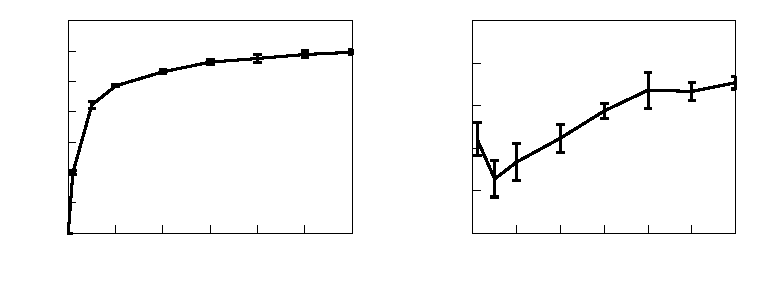
\includegraphics{hmc-mof5}}%
    \gplfronttext
  \end{picture}%
\endgroup

    \caption{Hybrid Grand Canonical Monte Carlo simulations results for the
    adsorption of methane in a simplified MOF-5 model. (left) adsorption
    isotherm at \SI{300}{K}, (right) volumes changes during adsorption.}
    \label{fig:hmc-mof5}
\end{figure}

The resulting isotherm is a simple type I isotherm, as expected for the
adsorption of methane in MOF-5. More interesting is the non-monotonous behavior
of the curve of volume deformations as a function of pressure. We first see a
small contraction of the unit cell at low loading, before the expected increase
at higher pressures. This contract--expand behavior is reminiscent of
sorption-induced deformation in other porous materials\cite{Balzer2013,
Mouhat2015}: the presence of few molecules inside the pores induces a
\emph{softening} and a contraction of the whole system. Another way to look at
this phenomenon is to envision the molecules inside the pore \emph{pulling} on
the pores wall.

=> bad model, good physics

=> needs electrostatics to go further

\newpage
\section{Computation of electrostatic energy in classical simulations}
\label{sec:electrostatic}

\subsection{The problem}

PBC: infinite + non convergence of the error if cutoff used

\subsection{Ewald summation}

Periodic: Fourier Transform!

\subsection{Wolf summation}

Papier originel de la méthode de Wolf\cite{Wolf1999}: on utilise le fait que le
potentiel effectif d'un multipole complexe est de l'ordre de $1/r^5$ pour
effectuer le calcul de l'énergie de Madelung via un simple somme de paires avec
un terme correctif. Ceci est équivalent à l'utilisation d'un potentiel
\emph{shifté}:
\[V_{SP}(r) = q_i q_j \left(\frac{1}{r} - \frac{1}{r_c} \right) \text{pour } r < r_c\]

Pour ne pas avoir besoin de rayons de coupure énormes, on utilse un potentiel amorti:
\[V_{DSP}(r) = \frac{q_i q_j \ \erfc(\alpha r)}{r} - \lim_{r \to r_c} \frac{q_i q_j \ \erfc(\alpha r)}{r}\]
\[\vec f_{ij}^{\ DSP} = q_i q_j \left[\frac{\erfc(\alpha r)}{r^2} + \frac{2\alpha}{\sqrt{\pi}} \frac{\exp(-\alpha^2 r^2)}{r}\right] \frac{\vec r}{r}
- q_i q_j \left[\frac{\erfc(\alpha R_c)}{R_c^2} + \frac{2\alpha}{\sqrt{\pi}} \frac{\exp(-\alpha^2 R_c^2)}{R_c}\right] \frac{\vec r}{r}\]


Les formules ci-dessus ont l'inconvénient de ne pas être $\mathcal{C}^1$ en $r_c$. Ce
papier\cite{Fennell2006} propose de partir de la force, et d'intégrer pour obtenir le potentiel
correspondant. On obtient:

\[\vec f_{ij}^{\ DSF} = q_i q_j \left[\frac{\erfc(\alpha r)}{r^2} + \frac{2\alpha}{\sqrt{\pi}} \frac{\exp(-\alpha^2 r^2)}{r}\right] \frac{\vec r}{r}
- q_i q_j \left[\frac{\erfc(\alpha R_c)}{R_c^2} + \frac{2\alpha}{\sqrt{\pi}} \frac{\exp(-\alpha^2 R_c^2)}{R_c}\right] \frac{\vec r}{r}\]

\[V_{DSF}(r) = q_i q_j \left[\frac{\erfc(\alpha r)}{r} - \frac{\erfc(\alpha r_c)}{r_c}
+ \left(\frac{\erfc(\alpha r_c)}{r_c^2} + \frac{2\alpha}{\sqrt{\pi}} \frac{\exp(-\alpha^2 r_c^2)}{r_c}\right) (r - r_c)\right]\]


\TODO \cite{Fukuda2013}

\subsection{Comparing Ewald and Wolf}

\OnlyInSubfile{\printbibliography}

\end{document}
